This section shows how the components run and interact in the system, by using Sequence Diagrams.

\subsubsection{Application Opening}

	This Sequence Diagram represents the first operations of \textit{Travlendar+}.
	When application is opened, the \textsl{Auto Login} procedure in the 'Access Manager' (see figure \ref{accessManagerDetail}) takes place: the 'Autentication Manager' checks for 'previously accesses data' in 'Saved Data Login' component. If the User has logged before, the User View is logged as explained later.
	On the contrary the \textsl{Login Page} of 'Guest View' of 'Mobile Application' component  (see figure \ref{mobileApplicationDetail}) is loaded.
	
	On this page the User, if already registered, he must fill the login form with his credential.
	'Autentication Manager' connects then to the 'DMBS' -contained in '\textit{Travlendar} Server' (see figure \ref{serverDetail})- in order to check if the form is properly compiled.
	
	'DBMS' returns a Result; if the credential are correct 'Autentication Manager' notifies Guest of the success of the procedure, and saves the aforementioned data to the 'Saved Data Login' component.
	
	Then a the \textsl{Content Recreation} procedure starts:
	'Profile Manager' component -contained in 'Application Aggregator' (see figure \ref{applicationAggregatorDetail})- loads all the necessary information about the User, and makes 'Calendar Manager' load all the informations about Appointments, Trips, and Breaks of the User; if necessary, 'Calendar Manager' and 'Preference Manager' (see figure \ref{preferenceManagerDetail}) have to restore them from the 'DBMS'.
	After all the data are loaded, the component 'User View' in 'Mobile Application' is told to show the \textsl{MainPage} to the User.
	
	In case of incorrect credentials, 'Autentication Manager' make the 'Guest View' notify the User of the not well compiled form, and makes him try again until the insertion of correct credentials.
	
	\begin{figure}[H]
		\centering
		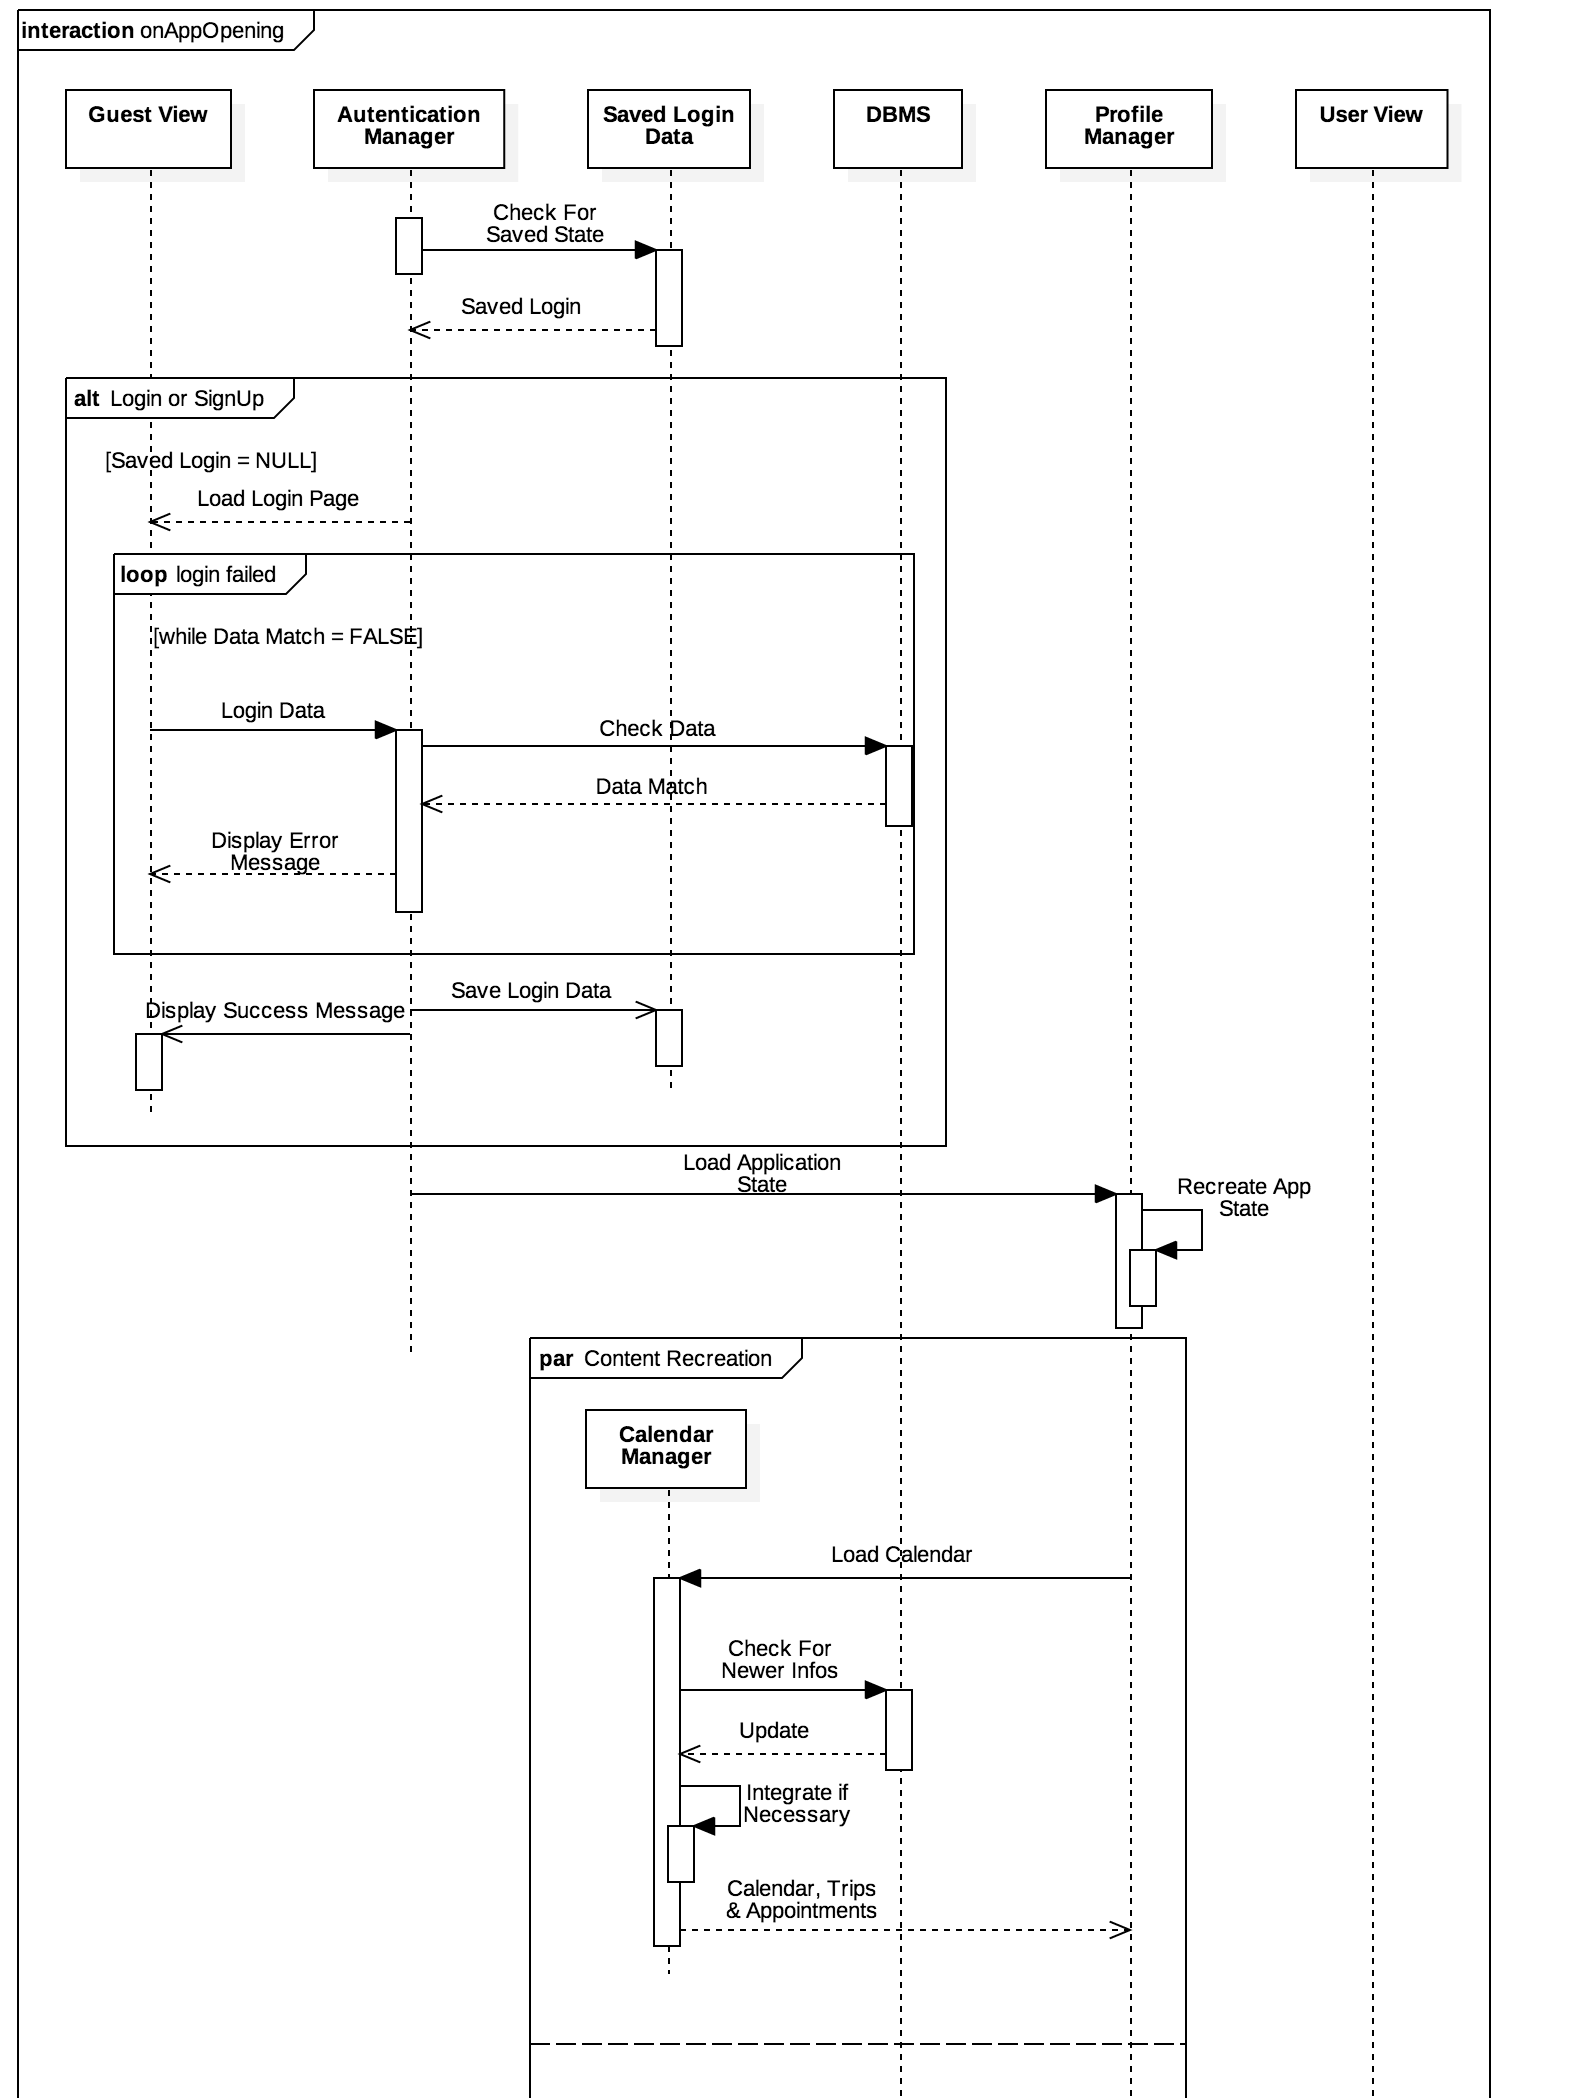
\includegraphics[width=0.9\textwidth]{UML/runtimeView/onOpening-part1}
		\caption{First Part of Application Opening Sequence Diagram}
	\end{figure}
	
	\vfill
	
	\begin{figure}[ht!]\ContinuedFloat
		\centering
		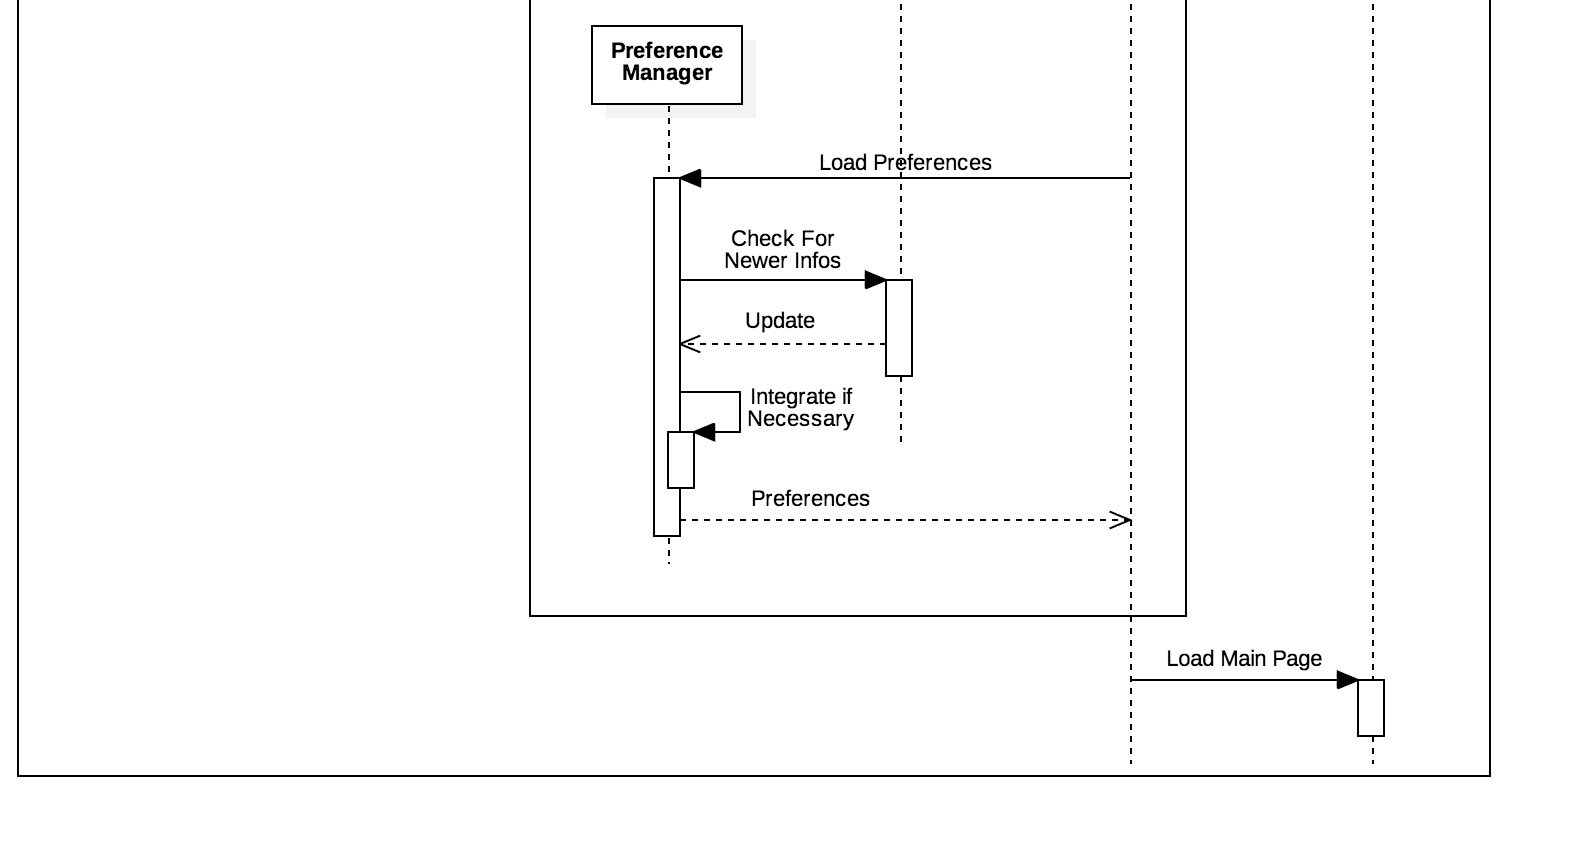
\includegraphics[width=0.9\textwidth]{UML/runtimeView/onOpening-part2}
		\caption{Second Part of Application Opening Sequence Diagram}
		\label{loginRunTimeView}
	\end{figure}
	

\subsubsection{Event Solutions Refreshing}
	
	This Sequence Diagram shows the reletaion between component when User tries to refresh or re-calculate already scheduled solutions for an Appointment.
	'User Action Handler' component  -contained in 'Application Aggregator' (see figure \ref{applicationAggregatorDetail})- receives the User's comand, and tells the 'Appoinemnt Aggregator' component -contained in 'Calendar Manager' component (see figure \ref{calendarManagerDetail})- to start the \textsl{Refreshing} procedure:
	All the Trip scheduled for the Appointment are taken from the 'Trip List' component, and are passed to the 'Scheduler' component  -contained in 'Travel Logic' component (see figure \ref{travelLogicDetail})-  in order to be confirmed o rescheduled.
	
	'Scheduler' has to consult, Excluded Vehicles, Maximum Time per Vehicle, Carbon Footprint and any other possibile preference defined by the User
	
	On the same time, 'Scheduler' contacts the 'API Request Distpatcher' of the '\textit{Travlendar} Server' component (see figure \ref{serverDetail}) in order to get all the external information about the Trip, like Public Transportation Timetable, Sharing Mean Position, Weather, and any other usefull detail.
	'API Request Distpatcher' sends a request 'API Manager' (see figure \ref{APIManagerDetail}) that, through his 'Listener' contacts all the necessary external APIs, and returns the 'Scheduler' requested information.
	All the Trip detail are passed to the 'Trip Handler' that is encharged of creating the new trip; the possible sequence of actions is shown in the RASD.
	
	If Purchasing is required 'Trip Handler' calls the 'Payment Handler' component  -contained in 'Payment Manager' (see figure \ref{paymentManagerDetail})-; this component is encharged to open the external Application and passing all the necessary informations in order to make User purchase requested service.
	After procedure is completed, the external Application returns to 'Payment Handler' that store the result in 'Purchase History' component, whatever the outcome is.
	Indeed that if the Purchase Procedure fails, is assumed that it will be re-tried in a second time, or a new Transportation Mean will be found, with the same sequence of actions shown in the RASD.
	
	The just created Trip is then passed to 'Calendar Manager', that notifies the User of the calendar updates via 'User Action Handler' and 'User View', and contacts the 'DMBS' of '\textit{Travlendar} Server' in order to store the new Trip.
	
	
	\begin{figure}[H]
		\centering
		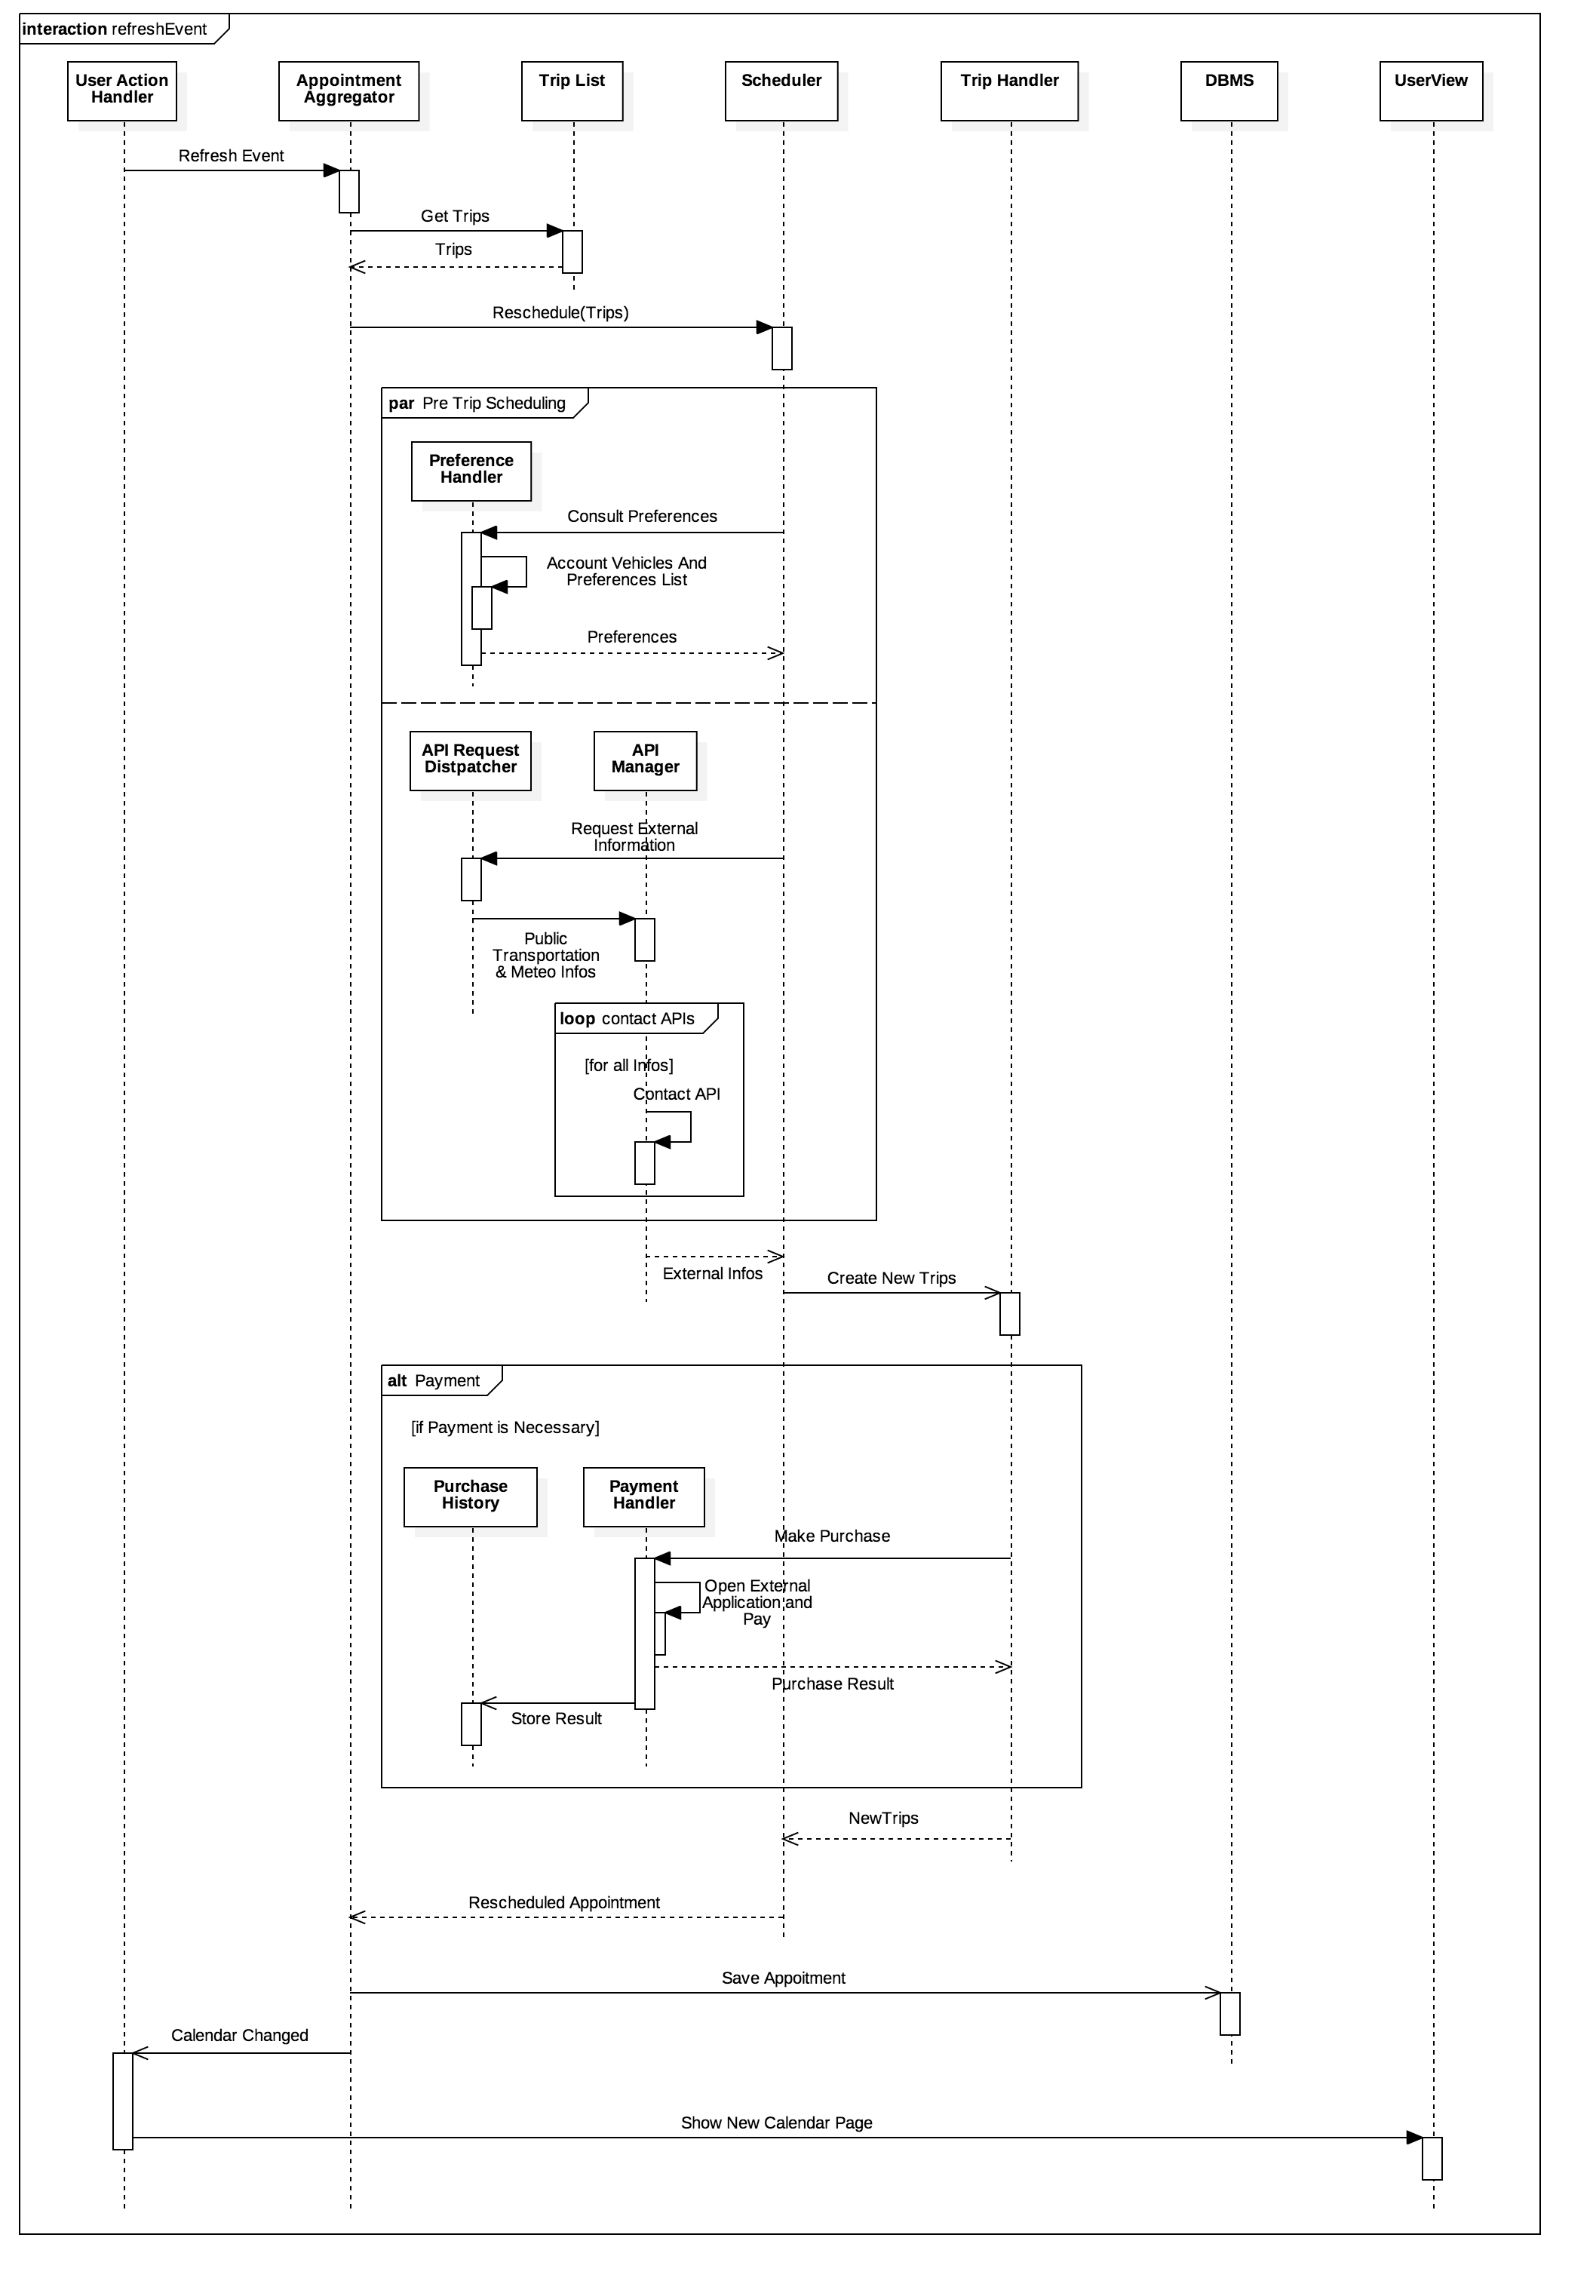
\includegraphics[width=0.9\textwidth]{UML/runtimeView/refreshEvent}
		\caption{Event Refreshing Sequence Diagram}
		\label{refreshRunTimeView}
	\end{figure}
	
	
	
